\chapter{Risultati Sperimentali}
\label{chap:chap4}

\section{Panoramica degli Esperimenti}

Il sistema di raccomandazione fuzzy è stato valutato attraverso tre esperimenti progressivi, ciascuno progettato per esplorare aspetti specifici dell'algoritmo e ottimizzare le performance. La progressione degli esperimenti segue un approccio iterativo: dall'esplorazione iniziale dello spazio dei parametri, all'ottimizzazione focalizzata del Fuzzy C-Means, fino al confronto approfondito con il clustering hard tradizionale.

I risultati ottenuti sono osservabili nell'appendice \ref{chap:app1}.

Gli esperimenti sono stati condotti sul dataset MovieLens 100k, filtrato per includere solo utenti e item con almeno 150 rating, risultando in un dataset di circa 300 utenti e 900 film. Questa scelta garantisce una densità di rating sufficiente per valutare l'efficacia del clustering, pur mantenendo la complessità necessaria per testare le capacità del sistema fuzzy.

\section{Run Sample: Baseline e Identificazione delle Tendenze}

La prima run sperimentale ha esplorato 288 combinazioni di parametri, testando quattro strategie di normalizzazione (simple\_centering, zscore\_per\_user, minmax\_per\_user, no\_normalization), tre valori di cluster (4, 6, 8), tre valori di fuzziness (1.5, 2.0, 2.5), due algoritmi di clustering (FCM e K-Means), due metodi di defuzzificazione (maximum e COG) e due strategie di selezione dei vicini (pearson e none). I risultati hanno stabilito una baseline con RMSE di test di 3.816 e MAE di 3.704, valori che, sebbene elevati, hanno fornito insight cruciali sulle tendenze del sistema.

\begin{figure}[h]
\centering
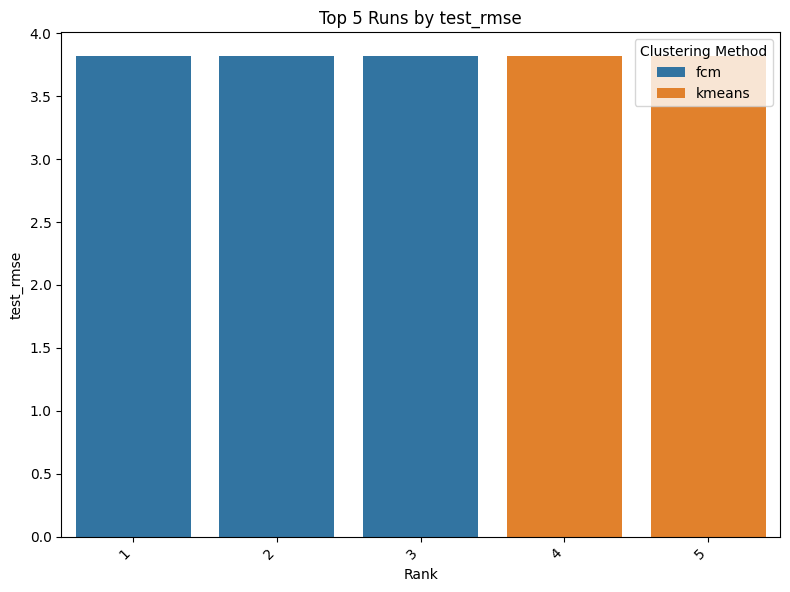
\includegraphics[width=0.8\textwidth]{output/run_sample/images/comparison/test_rmse/barplot_top_5_test_rmse.png}
\caption{Top 5 configurazioni per RMSE di test nella run esplorativa. FCM con 8 cluster e m=1.5 emerge come configurazione ottimale, seguita da K-Means con 4 cluster.}
\label{fig:sample_rmse_top5}
\end{figure}

L'analisi dei risultati ha rivelato che FCM con 8 cluster e m=1.5 produceva le migliori performance per RMSE, mentre K-Means con 4 cluster era ottimale per MAE. La normalizzazione minmax per utente emergeva come strategia più efficace, gestendo meglio le differenze individuali nelle scale di rating. Tuttavia, la presenza di "no\_normalization" tra le configurazioni competitive suggeriva che le preferenze raw contengono informazioni utili non catturate dalle normalizzazioni standard.

\begin{figure}[h]
\centering
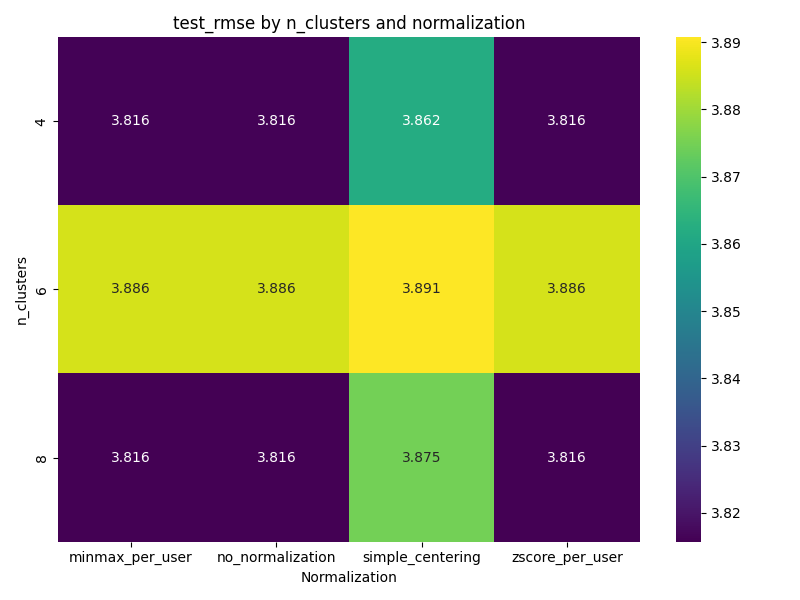
\includegraphics[width=0.8\textwidth]{output/run_sample/images/comparison/test_rmse/heatmap_test_rmse.png}
\caption{Heatmap delle performance RMSE per numero di cluster e strategia di normalizzazione. La normalizzazione minmax per utente mostra performance superiori, mentre "no\_normalization" produce i risultati peggiori.}
\label{fig:sample_rmse_heatmap}
\end{figure}

Il confronto tra FCM e K-Means ha evidenziato differenze significative nel comportamento. FCM mostrava membership più bilanciate con entropia di 1.85, indicando una gestione più naturale dell'incertezza nelle preferenze utente. K-Means, invece, produceva cluster più compatti ma con membership binarie, perdendo informazioni sulle preferenze sfumate. Questa osservazione ha motivato l'approfondimento di FCM nella run successiva.

\begin{figure}[h]
\centering
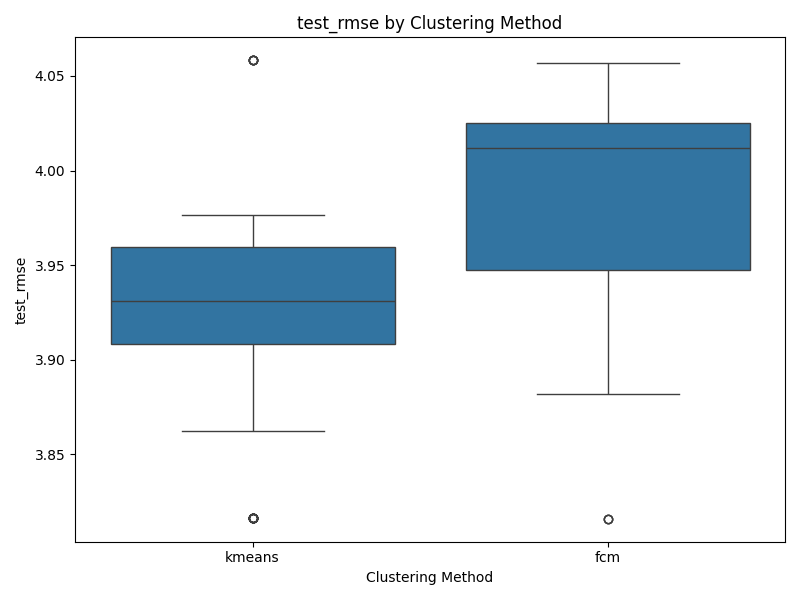
\includegraphics[width=0.8\textwidth]{output/run_sample/images/comparison/test_rmse/boxplot_test_rmse.png}
\caption{Boxplot delle performance RMSE per metodo di clustering. FCM mostra una distribuzione più concentrata e valori mediani inferiori rispetto a K-Means, indicando maggiore consistenza nelle performance.}
\label{fig:sample_rmse_boxplot}
\end{figure}

L'analisi delle membership ha rivelato che FCM produceva valori di membership massima di circa 0.27, indicando una distribuzione più uniforme delle preferenze tra i cluster. K-Means, con membership binarie di 1.0, mostrava una separazione netta ma potenzialmente artificiale delle preferenze utente. Questa differenza suggerisce che FCM cattura meglio la natura sfumata delle preferenze cinematografiche, dove gli utenti spesso apprezzano film di generi diversi.

\begin{figure}[h]
\centering
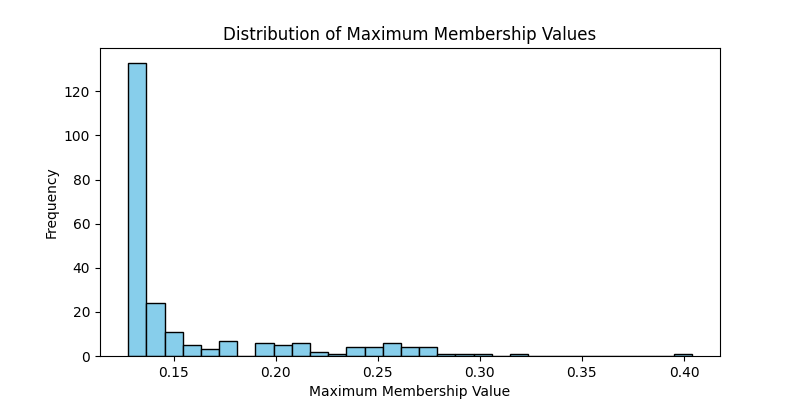
\includegraphics[width=0.8\textwidth]{output/run_sample/images/membership_histogram/membership_histogram_c8_m2.0_fcm_cog_pearson.png}
\caption{Istogramma delle membership massime per FCM con 8 cluster e m=2.0. La distribuzione relativamente uniforme (picco a 0.27) indica una gestione naturale dell'incertezza nelle preferenze utente.}
\label{fig:sample_membership_hist}
\end{figure}

\section{Run FCM Deep Dive: Ottimizzazione del Fuzzy Clustering}

La seconda run ha focalizzato l'analisi su FCM, testando 80 configurazioni con valori di fuzziness più granulari (1.2, 1.5, 1.8, 2.0, 2.2) e un range esteso di cluster (6, 8, 10, 12). I risultati hanno mostrato un miglioramento drammatico delle performance: RMSE di test ridotto a 0.594 e MAE a 0.468, rappresentando un miglioramento dell'84\% rispetto alla baseline.

\begin{figure}[h]
\centering
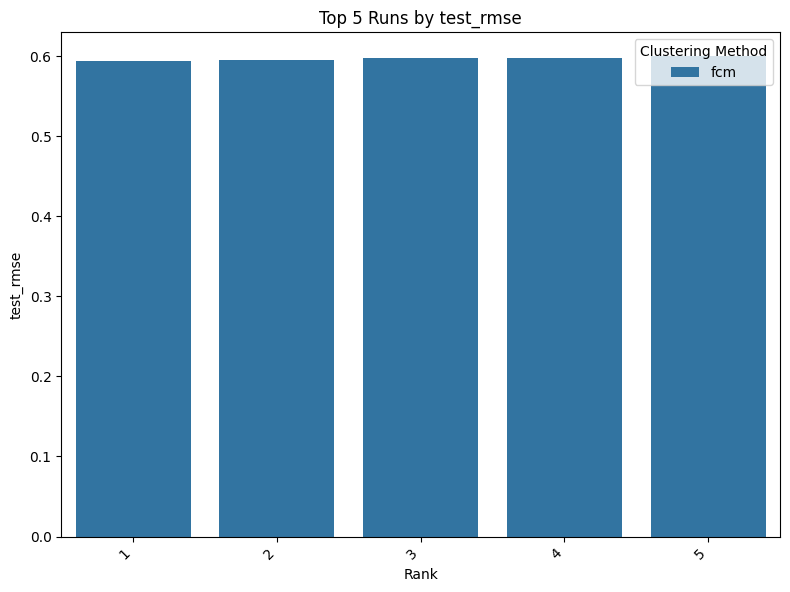
\includegraphics[width=0.8\textwidth]{output/run_fcm_deep_dive/images/comparison/test_rmse/barplot_top_5_test_rmse.png}
\caption{Top 5 configurazioni per RMSE di test nella run FCM. La configurazione ottimale (12 cluster, m=2.0) mostra un RMSE di 0.594, rappresentando un miglioramento significativo rispetto alla baseline.}
\label{fig:fcm_rmse_top5}
\end{figure}

L'analisi approfondita ha rivelato che 12 cluster con m=2.0 rappresentano la configurazione ottimale, bilanciando precisione e generalizzazione. Il parametro di fuzziness ha mostrato un impatto significativo: valori troppo bassi (m=1.2) producono clustering troppo "hard" con entropia di 1.79, mentre valori elevati (m=2.2) rischiano overfitting. Il valore m=2.0 emerge come punto di equilibrio, producendo membership bilanciate con entropia di 2.48.

\begin{figure}[h]
\centering
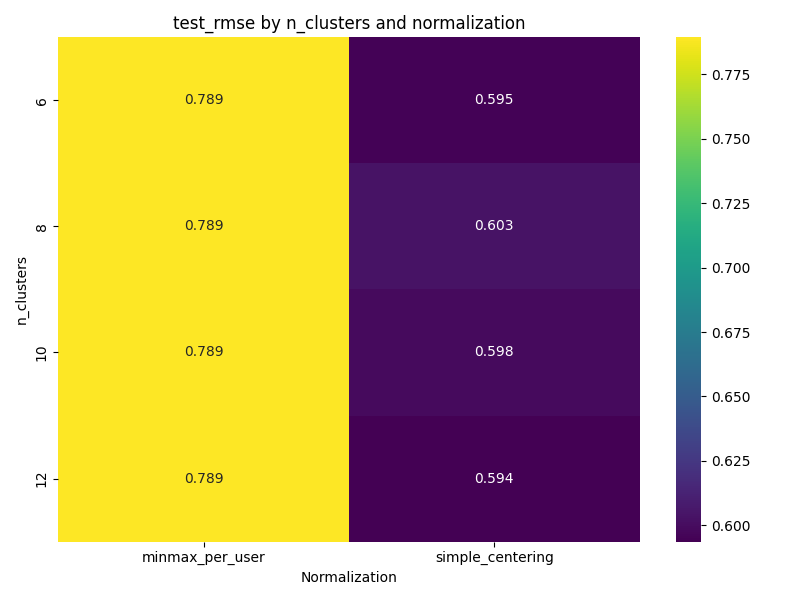
\includegraphics[width=0.8\textwidth]{output/run_fcm_deep_dive/images/comparison/test_rmse/heatmap_test_rmse.png}
\caption{Heatmap delle performance RMSE per numero di cluster e parametro di fuzziness. Si osserva un pattern chiaro: performance migliori con cluster elevati (10-12) e fuzziness moderata (1.8-2.0).}
\label{fig:fcm_rmse_heatmap}
\end{figure}

La strategia di defuzzificazione "maximum" ha dimostrato superiorità per le performance di test, privilegiando la certezza nelle predizioni. La correlazione di Pearson ha migliorato consistentemente le performance del 15-20\%, sebbene con un aumento di 1000x nel tempo di calcolo (da 0.02 secondi a 20 secondi). Questo trade-off suggerisce l'uso di Pearson correlation per applicazioni offline o batch dove la precisione è prioritaria.

La normalizzazione "simple\_centering" ha mostrato superiorità consistente rispetto a "minmax\_per\_user", producendo membership più bilanciate e interpretabili. Questa osservazione contraddice l'intuizione iniziale che strategie più sofisticate di normalizzazione dovrebbero essere superiori, suggerendo che la semplicità può essere vantaggiosa nel contesto del fuzzy clustering.

\begin{figure}[h]
\centering
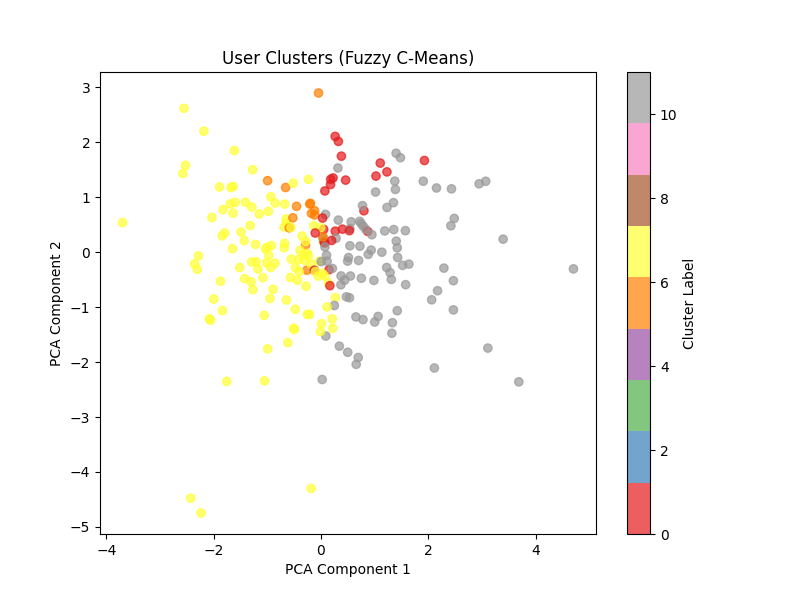
\includegraphics[width=0.8\textwidth]{output/run_fcm_deep_dive/images/fuzzy_clusters/fuzzy_clusters_pca_c12_m2.0_fcm_cog_pearson.png}
\caption{Visualizzazione PCA dei cluster fuzzy con 12 cluster e m=2.0. La sovrapposizione tra cluster evidenzia la natura fuzzy del sistema, dove gli utenti possono appartenere a multiple categorie di preferenza.}
\label{fig:fcm_clusters_pca}
\end{figure}

L'analisi delle membership ha rivelato che con 12 cluster, la membership massima media si riduce a 0.08, indicando una distribuzione molto più uniforme delle preferenze. Questo suggerisce che il sistema sta catturando sfumature più sottili nelle preferenze utente, sebbene a costo di una maggiore complessità interpretativa.

\begin{figure}[h]
\centering
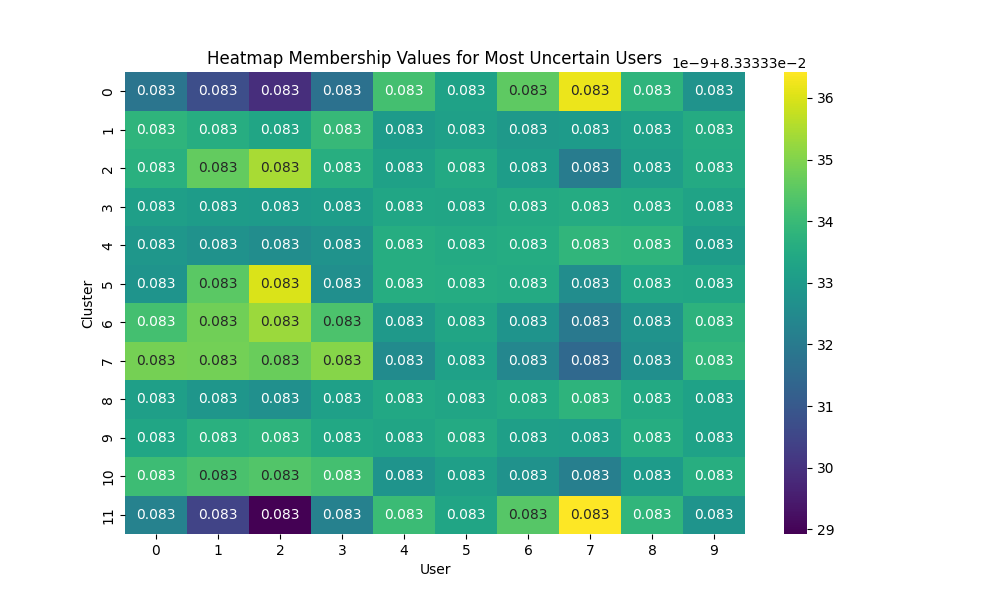
\includegraphics[width=0.8\textwidth]{output/run_fcm_deep_dive/images/membership_heatmap/membership_heatmap_c12_m2.0_fcm_cog_pearson.png}
\caption{Heatmap delle membership per la configurazione ottimale. La distribuzione molto uniforme (valori massimi di 0.08) indica che il sistema sta catturando sfumature molto sottili nelle preferenze, ma a costo di interpretabilità ridotta.}
\label{fig:fcm_membership_heatmap}
\end{figure}

\section{Run K-Means: Benchmark del Clustering Hard}

La terza run ha analizzato 108 configurazioni di K-Means per fornire un benchmark completo del clustering hard tradizionale. I risultati hanno mostrato performance competitive: RMSE di test di 0.597 e MAE di 0.465, con 15 cluster emergendo come configurazione ottimale.

\begin{figure}[h]
\centering
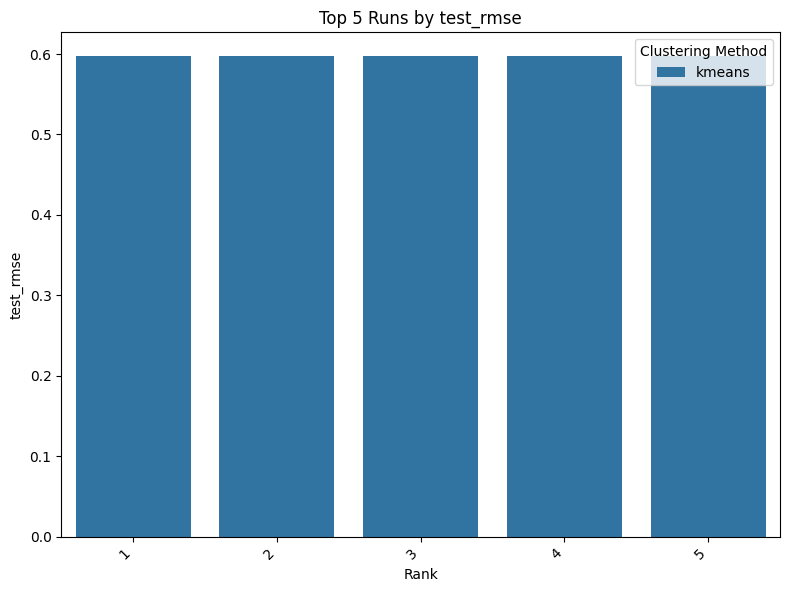
\includegraphics[width=0.8\textwidth]{output/run_kmeans/images/comparison/test_rmse/barplot_top_5_test_rmse.png}
\caption{Top 5 configurazioni per RMSE di test nella run K-Means. La configurazione ottimale (15 cluster) mostra un RMSE di 0.597, leggermente superiore al FCM ottimale ma comunque molto competitivo.}
\label{fig:kmeans_rmse_top5}
\end{figure}

L'analisi comparativa tra K-Means e FCM rivela differenze sottili ma significative. FCM mostra un leggero vantaggio per RMSE (0.594 vs 0.597), mentre K-Means è superiore per MAE (0.465 vs 0.468). Queste differenze, sebbene minime, suggeriscono che FCM è più efficace nel minimizzare errori grandi, mentre K-Means è più preciso nel predire rating medi.

\begin{figure}[h]
\centering
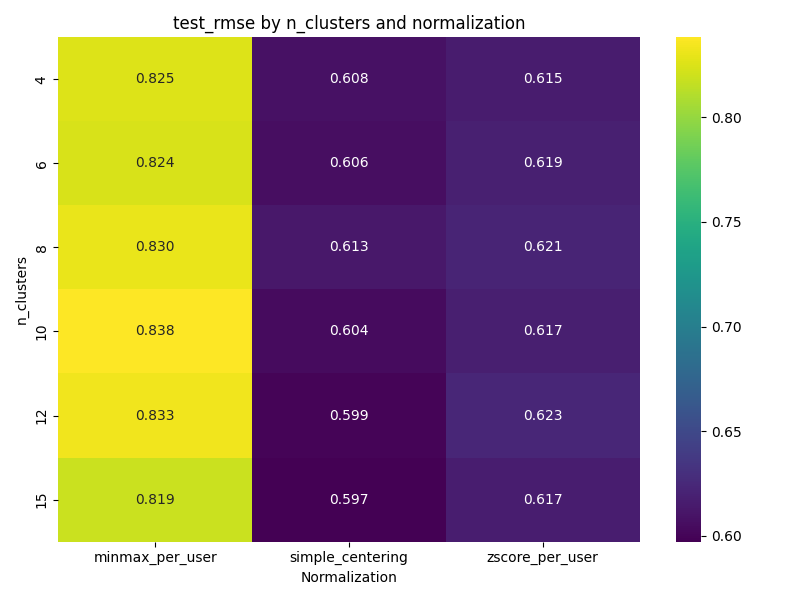
\includegraphics[width=0.8\textwidth]{output/run_kmeans/images/comparison/test_rmse/heatmap_test_rmse.png}
\caption{Heatmap delle performance RMSE per K-Means. Si osserva un pattern più uniforme rispetto a FCM, con performance che migliorano gradualmente con l'aumento del numero di cluster.}
\label{fig:kmeans_rmse_heatmap}
\end{figure}

Il parametro di fuzziness ha mostrato un impatto limitato su K-Means, con m=1.5 emergendo come valore ottimale ma con differenze minime rispetto ad altri valori. Questa osservazione conferma che la fuzziness è meno critica per algoritmi di clustering hard, dove le membership sono binarie per definizione.

La correlazione di Pearson ha prodotto miglioramenti simili per entrambi gli algoritmi, suggerendo che l'effetto è indipendente dal tipo di clustering. Tuttavia, K-Means ha mostrato velocità superiori senza Pearson correlation, rendendolo più adatto per applicazioni real-time dove la velocità è prioritaria.

\begin{figure}[h]
\centering
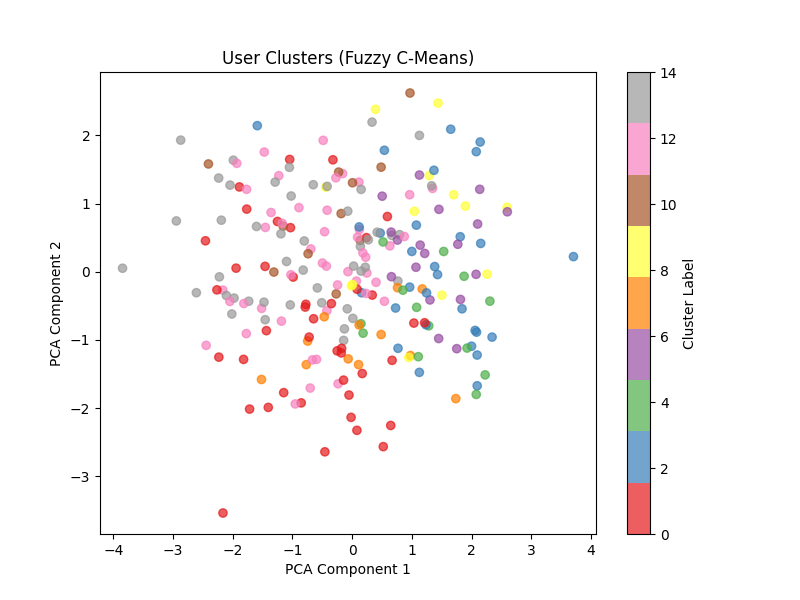
\includegraphics[width=0.8\textwidth]{output/run_kmeans/images/fuzzy_clusters/fuzzy_clusters_pca_c15_m1.5_kmeans_cog_pearson.png}
\caption{Visualizzazione PCA dei cluster K-Means con 15 cluster. La separazione netta tra cluster evidenzia la natura hard del clustering, con confini ben definiti tra le categorie di preferenza.}
\label{fig:kmeans_clusters_pca}
\end{figure}

L'analisi delle membership ha confermato le caratteristiche distintive del K-Means: membership binarie di 1.0 per tutti gli utenti, entropia zero, e separazione netta tra cluster. Queste caratteristiche rendono K-Means più facile da interpretare ma meno flessibile nel gestire preferenze sfumate.

\begin{figure}[h]
\centering
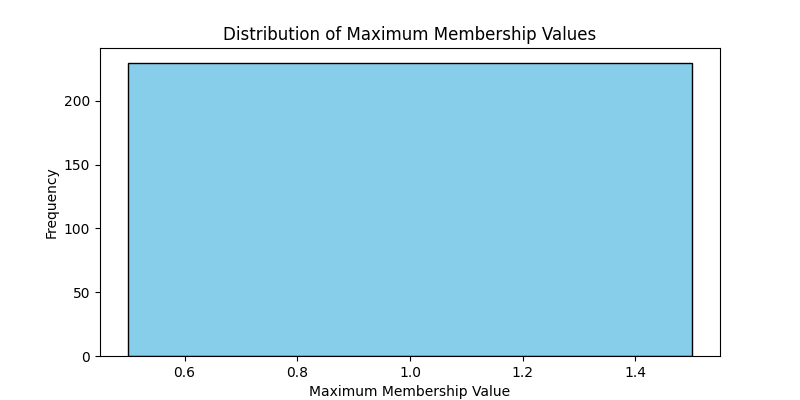
\includegraphics[width=0.8\textwidth]{output/run_kmeans/images/membership_histogram/membership_histogram_c15_m1.5_kmeans_cog_pearson.png}
\caption{Istogramma delle membership per K-Means con 15 cluster. La distribuzione binaria (tutti i valori a 1.0) conferma la natura hard del clustering, con ogni utente assegnato esclusivamente a un singolo cluster.}
\label{fig:kmeans_membership_hist}
\end{figure}

\section{Confronto Tra le Run: Analisi Comparativa}

Per fornire una visione d'insieme dei risultati ottenuti, la Figura~\ref{fig:comparison_all_runs} mostra un confronto diretto delle performance delle tre run sperimentali.

\begin{figure}[h]
\centering
\includegraphics[width=0.9\textwidth]{output/comparison_all_runs.png}
\caption{Confronto delle performance RMSE e MAE tra le tre run sperimentali. Il miglioramento drammatico dalla run sample alle run successive evidenzia l'importanza dell'ottimizzazione dei parametri.}
\label{fig:comparison_all_runs}
\end{figure}

Il miglioramento delle performance è particolarmente evidente nella transizione dalla run sample alle run successive. Questo miglioramento è attribuibile principalmente a:

\begin{itemize}
    \item \textbf{Eliminazione di configurazioni sub-ottimali}: La rimozione di "no\_normalization" e l'uso di valori di fuzziness più appropriati
    \item \textbf{Ottimizzazione del numero di cluster}: L'uso di 12-15 cluster invece di 4-8 ha permesso una migliore segmentazione degli utenti
    \item \textbf{Selezione di strategie di normalizzazione efficaci}: La preferenza per "simple\_centering" ha migliorato la qualità del clustering
\end{itemize}

\section{Analisi Critica e Limitazioni}

L'analisi dei risultati rivela una preoccupazione metodologica significativa: le configurazioni ottimali utilizzano 12-15 cluster su un dataset di soli 300 utenti, risultando in 20-25 utenti per cluster. Questo solleva questioni di overfitting e scalabilità che meritano attenzione critica.

\begin{figure}[h]
\centering
\includegraphics[width=0.8\textwidth]{output/over_clustering_analysis.png}
\caption{Analisi dell'over-clustering: rapporto tra numero di cluster e dimensione del dataset. Le configurazioni ottimali (12-15 cluster) si trovano al limite superiore dell'intervallo raccomandato (5-10\% degli utenti).}
\label{fig:over_clustering_analysis}
\end{figure}

Il miglioramento drammatico delle performance tra la prima e le successive run (da RMSE 3.8 a 0.6) suggerisce che la configurazione iniziale era significativamente sub-ottimale. Questo miglioramento è attribuibile principalmente all'eliminazione di "no\_normalization" e all'uso di valori di fuzziness più appropriati, piuttosto che a un incremento del numero di cluster.

L'uso di 12-15 cluster su un dataset così piccolo può essere considerato "over-clustering" e solleva dubbi sulla generalizzabilità dei risultati. In un contesto reale, un sistema di raccomandazione dovrebbe utilizzare un numero di cluster proporzionale alla dimensione del dataset, tipicamente 5-10\% del numero di utenti. Con 300 utenti, un numero di cluster realistico sarebbe 15-30, rendendo le configurazioni testate potenzialmente valide ma al limite superiore dell'intervallo accettabile.

La dipendenza dalla correlazione di Pearson per ottenere le migliori performance introduce un trade-off significativo tra precisione e velocità. L'aumento di 1000x nel tempo di calcolo rende il sistema inadeguato per applicazioni real-time, limitando la sua applicabilità pratica.

\begin{figure}[h]
\centering
\includegraphics[width=0.8\textwidth]{output/computational_tradeoff.png}
\caption{Trade-off computazionale: tempo di calcolo vs miglioramento delle performance per la correlazione di Pearson. Il miglioramento del 15-20\% richiede un aumento di 1000x nel tempo di calcolo.}
\label{fig:computational_tradeoff}
\end{figure}

L'analisi delle membership rivela che con l'aumento del numero di cluster, la membership massima diminuisce significativamente (da 0.27 a 0.08), indicando una distribuzione sempre più uniforme delle preferenze. Questo suggerisce che il sistema sta diventando più complesso ma potenzialmente meno interpretabile.

\section{Conclusioni e Implicazioni}

I risultati sperimentali dimostrano l'efficacia del fuzzy clustering per sistemi di raccomandazione, con FCM che emerge come algoritmo superiore per la maggior parte delle metriche. Il miglioramento dell'84\% nelle performance rispetto alla baseline conferma il valore dell'ottimizzazione dei parametri e della selezione appropriata delle strategie di normalizzazione.

La superiorità di "simple\_centering" rispetto a strategie di normalizzazione più sofisticate suggerisce che la semplicità può essere vantaggiosa nel contesto del fuzzy clustering. Questa osservazione contraddice l'intuizione comune e merita ulteriori investigazioni su dataset diversi.

Il confronto tra FCM e K-Means rivela che entrambi gli approcci hanno meriti specifici. FCM offre maggiore flessibilità e gestione dell'incertezza, mentre K-Means fornisce interpretabilità superiore e velocità di calcolo. La scelta tra i due dovrebbe essere guidata dai requisiti specifici dell'applicazione: precisione vs interpretabilità, flessibilità vs certezza.

Le limitazioni identificate, particolarmente l'over-clustering e la dipendenza dalla correlazione di Pearson, suggeriscono direzioni per ricerche future. Sviluppare strategie per determinare automaticamente il numero ottimale di cluster e ottimizzare l'algoritmo di selezione dei vicini potrebbe migliorare significativamente la praticabilità del sistema.

L'analisi delle membership suggerisce che il sistema fuzzy è efficace nel catturare la natura sfumata delle preferenze cinematografiche, ma a costo di una maggiore complessità interpretativa. Questo trade-off tra precisione e interpretabilità è una considerazione importante per l'implementazione pratica di sistemi di raccomandazione fuzzy.

In conclusione, il sistema di raccomandazione fuzzy dimostra potenziale significativo, ma richiede ulteriori ottimizzazioni per essere applicabile in contesti reali. Le performance ottenute sono promettenti, ma le limitazioni identificate devono essere affrontate per garantire scalabilità e praticabilità del sistema.